\documentclass[10pt]{article}
\usepackage{geometry}                % See geometry.pdf to learn the layout options. There are lots.
\geometry{a4paper
}                   % ... or a4paper or a5paper or ... 
\usepackage[parfill]{parskip}    % Activate to begin paragraphs with an empty line rather than an indent

%%%%%%%%%%%%%%%%%%%%
\newcommand{\hide}[1]{}

\usepackage{natbib}
\usepackage{xcolor}
\usepackage{hyperref}
\usepackage{mathtools}
\usepackage{array}
\usepackage{multirow}
\usepackage{graphicx}
\usepackage{subcaption}
\usepackage{mwe}
\usepackage{float}
\usepackage{booktabs}
\usepackage{url}

\usepackage[T1]{fontenc}
\usepackage{tikz}
\usetikzlibrary{arrows.meta,positioning}



\title {CS31710 Advanced Algorithms}




\begin{document}
\maketitle

\section*{Task 1 - Introduction}

This assignment is about solving a rounding problem involving a matrix. You have a ZxZ grid of numbers and have to round each number so that the sums of the rows and columns are the same as in the original square. The sums of the rows and columns can also be rounded up or down. There may not always be valid rounding for every combination of numbers and the program needs to be able to cope with this as well. 

In the remainder of this report I will talk about how I modelled and solved this problem and discuss and evaluate my approach.

\section*{Task 2 - Modelling}

You want to model the matrix as a maximum flow problem. Each number in the matrix and each row and column sum need to have an edge so for a 3x3 matrix that would be 15 edges, every number needs an edge because edges are how you represent flow and demand in maximum flow problems. You can achieve this by having six nodes arranged in a 3x2 configuration, the first set of nodes represent the columns and the second set represent the rows. Each number has a lower bound and an upper bound and the edges need to reflect this so their flow will be restricted based on their demand, the lower bound, and their capacity, the upper bound. The source connects to the first set of three nodes and the sink connects to the last three.

Figure \ref{fig:maxflow} shows the left hand side example from the assignment brief. The source connects to three nodes; 1, 2 and 3, these nodes represent the columns and the edge connecting the source to the node represents the sum of each column. Each column then connects to three nodes; 4, 5 and 6, these edges represent the numbers in each column. Nodes 4, 5 and 6 connect to the sink and the sink connection represents the sum of the row.

Each edge has a flow variable which can take a value between its lower bound and its upper bound, if the number the edge is representing is an integer then the flow variable just has a rule that it is equal to that number. For example edge X01 in the list below is the variable that corresponds to the sum of the first column, because the sum of this column is 8, a whole number, then the constraint for this variable is that it is equal to 8. In the example graph in figure \ref{fig:maxflow} the flow constraints are:


\begin{itemize}
    
    \item X01 = 8
    \item X02 = 17
    \item X03  = 13
    
    \item 2 <= X11 <= 3
    \item 1 <= X12 <= 2
    \item 3 <= X13 <= 4
    
    \item 4 <= X21 <= 5
    \item  X22 = 5
    \item 7 <= X23 <= 8
    
    \item 8 <= X31 <= 9
    \item 3 <= X32 <= 4
    \item 1 <= X33 <= 2
    
    \item X41 = 16
    \item X51 = 10
    \item X61 = 12

\end{itemize}

There is also a constraint for each node because in a maximum flow problem what is flowing into a node must also be flowing out of it. These constraints will need to be equal to 0 before they can be put into GLPK.
\begin{itemize}
    \item X01 = X11 + X12 + X13
    \item X02 = X21 + X22 + X23
    \item X03 = X31 + X32 + X33
    \item X11 + X21 + X31 = X41
    \item X12 + X22 + X32 = X51
    \item X13 + X23 + X33 = X61
\end{itemize}

To turn this into a linear program you have to formulate the objective function, this function is the goal of the linear program and represents what it is trying to achieve. To do this you introduce an artificial flow from the sink back to the source, figure \ref{fig:circulationmaxflow} shows this. This turns it into a closed network and adds a new variable and two new constraints. The new variable is X71 which is the new edge and the constraints are X41 + X51 + X61 = X71 and X71 = X01 + X02 + X03. The objective function is simply to maximise X71 because you want to maximise the flow from the source to the sink.

So overall you have a constraint for every bounded edge and for every node, in this example that's 23 constraints. It can also be worked out as $size^2 + (size * 4) + 2$ and the number of variables is 16 and can be worked out as $size^2 + (size * 2) + 1$. Essentially every edge has a variable and every node and edge, except the one from the sink to the source, are constrained.

Therefore the linear program can be summarised as max X70 given:
\begin{itemize}
    \item X01 - X11 - X12 - X13 = 0
    \item X02 - X21 - X22 - X23 = 0
    \item X03 - X31 - X32 - X33 = 0
    \item X11 + X21 + X31 - X41 = 0
    \item X12 + X22 + X32 - X51 = 0
    \item X13 + X23 + X33 - X61 = 0
    \item X41 + X51 + X61 - X71 = 0
    \item X71 - X01 - X02 - X03 = 0
    
    \item X01 = 8
    \item X02 = 17
    \item X03  = 13
    
    \item 2 <= X11 <= 3
    \item 1 <= X12 <= 2
    \item 3 <= X13 <= 4
    
    \item 4 <= X21 <= 5
    \item  X22 = 5
    \item 7 <= X23 <= 8
    
    \item 8 <= X31 <= 9
    \item 3 <= X32 <= 4
    \item 1 <= X33 <= 2
    
    \item X41 = 16
    \item X51 = 10
    \item X61 = 12
\end{itemize}

In the program the variables map to these 
\begin{itemize}
    \item x1 = X01
    \item x2 = x02
    \item x3 = x03
    \item x4 = x11
    \item x5 = x12
    \item x6 = x13
    \item x7 = x21
    \item x8 = x22
    \item x9 = x23
    \item x10 = x31
    \item x11 = x32
    \item x12 = x33
    \item x13 = x41
    \item x14 = x51
    \item x15 = x61
    \item x16 = x71
\end{itemize}{}
So in the GLPK program you want to maximise x16.



\begin{figure}
\centering




\tikzset{every picture/.style={line width=0.75pt}} %set default line width to 0.75pt        

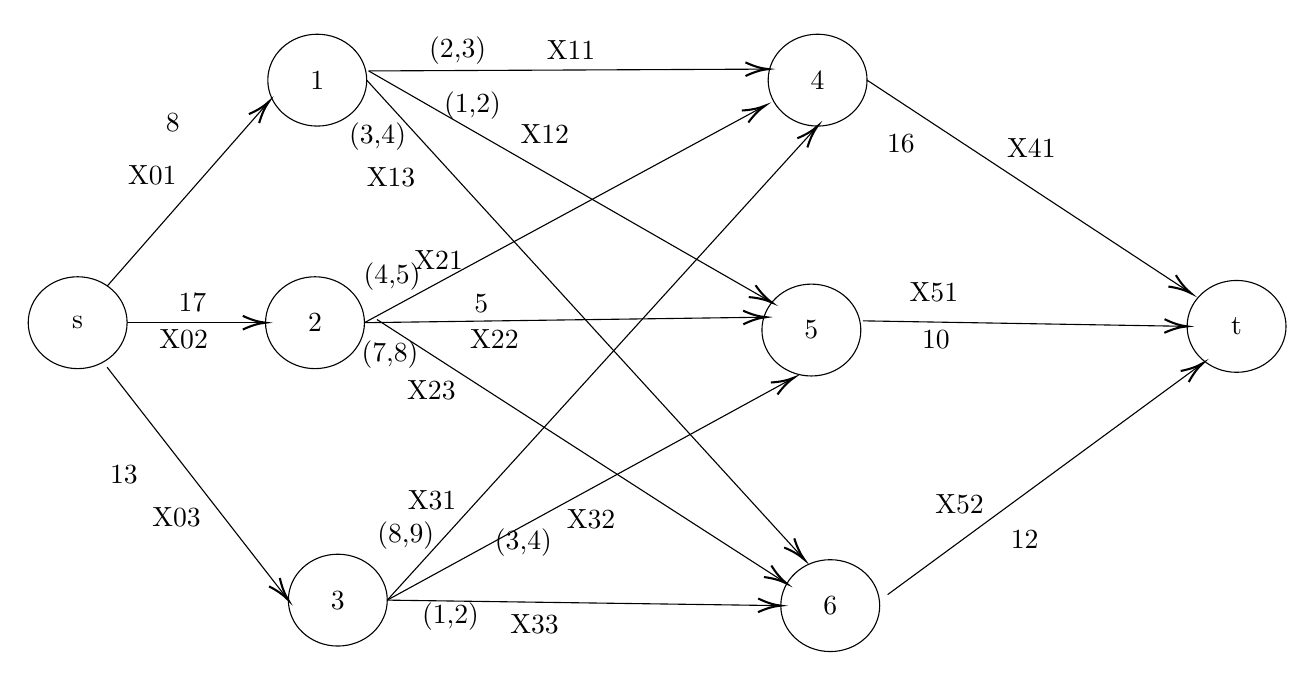
\begin{tikzpicture}[x=0.75pt,y=0.75pt,yscale=-1,xscale=1]
%uncomment if require: \path (0,328); %set diagram left start at 0, and has height of 328

%Shape: Ellipse [id:dp6087199415982871] 
\draw   (5,164.55) .. controls (5,152.33) and (15.66,142.42) .. (28.82,142.42) .. controls (41.98,142.42) and (52.64,152.33) .. (52.64,164.55) .. controls (52.64,176.77) and (41.98,186.68) .. (28.82,186.68) .. controls (15.66,186.68) and (5,176.77) .. (5,164.55) -- cycle ;
%Shape: Ellipse [id:dp6442628638464488] 
\draw   (120.43,47.69) .. controls (120.43,35.46) and (131.1,25.56) .. (144.25,25.56) .. controls (157.41,25.56) and (168.08,35.46) .. (168.08,47.69) .. controls (168.08,59.91) and (157.41,69.82) .. (144.25,69.82) .. controls (131.1,69.82) and (120.43,59.91) .. (120.43,47.69) -- cycle ;
%Shape: Ellipse [id:dp1061001134607138] 
\draw   (119.34,164.55) .. controls (119.34,152.33) and (130,142.42) .. (143.16,142.42) .. controls (156.32,142.42) and (166.98,152.33) .. (166.98,164.55) .. controls (166.98,176.77) and (156.32,186.68) .. (143.16,186.68) .. controls (130,186.68) and (119.34,176.77) .. (119.34,164.55) -- cycle ;
%Shape: Ellipse [id:dp07911004918526843] 
\draw   (130.34,298.21) .. controls (130.34,285.99) and (141,276.09) .. (154.16,276.09) .. controls (167.32,276.09) and (177.98,285.99) .. (177.98,298.21) .. controls (177.98,310.44) and (167.32,320.34) .. (154.16,320.34) .. controls (141,320.34) and (130.34,310.44) .. (130.34,298.21) -- cycle ;
%Shape: Ellipse [id:dp03846588488001945] 
\draw   (361.5,47.69) .. controls (361.5,35.46) and (372.16,25.56) .. (385.32,25.56) .. controls (398.48,25.56) and (409.14,35.46) .. (409.14,47.69) .. controls (409.14,59.91) and (398.48,69.82) .. (385.32,69.82) .. controls (372.16,69.82) and (361.5,59.91) .. (361.5,47.69) -- cycle ;
%Shape: Ellipse [id:dp6541338138904766] 
\draw   (358.5,168.09) .. controls (358.5,155.87) and (369.16,145.96) .. (382.32,145.96) .. controls (395.48,145.96) and (406.14,155.87) .. (406.14,168.09) .. controls (406.14,180.31) and (395.48,190.22) .. (382.32,190.22) .. controls (369.16,190.22) and (358.5,180.31) .. (358.5,168.09) -- cycle ;
%Shape: Ellipse [id:dp4549789345673577] 
\draw   (367.59,300.87) .. controls (367.59,288.65) and (378.26,278.74) .. (391.42,278.74) .. controls (404.57,278.74) and (415.24,288.65) .. (415.24,300.87) .. controls (415.24,313.09) and (404.57,323) .. (391.42,323) .. controls (378.26,323) and (367.59,313.09) .. (367.59,300.87) -- cycle ;
%Shape: Ellipse [id:dp8272562609322014] 
\draw   (563.36,166.32) .. controls (563.36,154.1) and (574.02,144.19) .. (587.18,144.19) .. controls (600.34,144.19) and (611,154.1) .. (611,166.32) .. controls (611,178.54) and (600.34,188.45) .. (587.18,188.45) .. controls (574.02,188.45) and (563.36,178.54) .. (563.36,166.32) -- cycle ;
%Straight Lines [id:da9018286841586965] 
\draw    (43.11,146.84) -- (119.68,59.5) ;
\draw [shift={(121,58)}, rotate = 491.24] [color={rgb, 255:red, 0; green, 0; blue, 0 }  ][line width=0.75]    (10.93,-3.29) .. controls (6.95,-1.4) and (3.31,-0.3) .. (0,0) .. controls (3.31,0.3) and (6.95,1.4) .. (10.93,3.29)   ;

%Straight Lines [id:da06248575236412646] 
\draw    (52.64,164.55) -- (117.34,164.55) ;
\draw [shift={(119.34,164.55)}, rotate = 180] [color={rgb, 255:red, 0; green, 0; blue, 0 }  ][line width=0.75]    (10.93,-3.29) .. controls (6.95,-1.4) and (3.31,-0.3) .. (0,0) .. controls (3.31,0.3) and (6.95,1.4) .. (10.93,3.29)   ;

%Straight Lines [id:da3422343152189683] 
\draw    (43,186) -- (129.11,296.64) ;
\draw [shift={(130.34,298.21)}, rotate = 232.11] [color={rgb, 255:red, 0; green, 0; blue, 0 }  ][line width=0.75]    (10.93,-3.29) .. controls (6.95,-1.4) and (3.31,-0.3) .. (0,0) .. controls (3.31,0.3) and (6.95,1.4) .. (10.93,3.29)   ;

%Straight Lines [id:da7764471766115765] 
\draw    (168.08,47.69) -- (377.68,277.26) ;
\draw [shift={(379.03,278.74)}, rotate = 227.6] [color={rgb, 255:red, 0; green, 0; blue, 0 }  ][line width=0.75]    (10.93,-3.29) .. controls (6.95,-1.4) and (3.31,-0.3) .. (0,0) .. controls (3.31,0.3) and (6.95,1.4) .. (10.93,3.29)   ;

%Straight Lines [id:da6708148744128288] 
\draw    (169.03,43.26) -- (359.5,42.38) ;
\draw [shift={(361.5,42.37)}, rotate = 539.74] [color={rgb, 255:red, 0; green, 0; blue, 0 }  ][line width=0.75]    (10.93,-3.29) .. controls (6.95,-1.4) and (3.31,-0.3) .. (0,0) .. controls (3.31,0.3) and (6.95,1.4) .. (10.93,3.29)   ;

%Straight Lines [id:da04844893541614448] 
\draw    (169.03,43.26) -- (361.53,153.82) ;
\draw [shift={(363.26,154.81)}, rotate = 209.87] [color={rgb, 255:red, 0; green, 0; blue, 0 }  ][line width=0.75]    (10.93,-3.29) .. controls (6.95,-1.4) and (3.31,-0.3) .. (0,0) .. controls (3.31,0.3) and (6.95,1.4) .. (10.93,3.29)   ;

%Straight Lines [id:da603114895121129] 
\draw    (166.98,164.55) -- (358.24,60.95) ;
\draw [shift={(360,60)}, rotate = 511.56] [color={rgb, 255:red, 0; green, 0; blue, 0 }  ][line width=0.75]    (10.93,-3.29) .. controls (6.95,-1.4) and (3.31,-0.3) .. (0,0) .. controls (3.31,0.3) and (6.95,1.4) .. (10.93,3.29)   ;

%Straight Lines [id:da2515352222135493] 
\draw    (166.98,164.55) -- (358.41,161.92) ;
\draw [shift={(360.41,161.89)}, rotate = 539.21] [color={rgb, 255:red, 0; green, 0; blue, 0 }  ][line width=0.75]    (10.93,-3.29) .. controls (6.95,-1.4) and (3.31,-0.3) .. (0,0) .. controls (3.31,0.3) and (6.95,1.4) .. (10.93,3.29)   ;

%Straight Lines [id:da18679069580618912] 
\draw    (173,163) -- (368.77,289.16) ;
\draw [shift={(370.45,290.25)}, rotate = 212.8] [color={rgb, 255:red, 0; green, 0; blue, 0 }  ][line width=0.75]    (10.93,-3.29) .. controls (6.95,-1.4) and (3.31,-0.3) .. (0,0) .. controls (3.31,0.3) and (6.95,1.4) .. (10.93,3.29)   ;

%Straight Lines [id:da5352286234985627] 
\draw    (177.98,298.21) -- (383.98,71.3) ;
\draw [shift={(385.32,69.82)}, rotate = 492.23] [color={rgb, 255:red, 0; green, 0; blue, 0 }  ][line width=0.75]    (10.93,-3.29) .. controls (6.95,-1.4) and (3.31,-0.3) .. (0,0) .. controls (3.31,0.3) and (6.95,1.4) .. (10.93,3.29)   ;

%Straight Lines [id:da24470161199444096] 
\draw    (177.98,298.21) -- (372.25,191.96) ;
\draw [shift={(374,191)}, rotate = 511.32] [color={rgb, 255:red, 0; green, 0; blue, 0 }  ][line width=0.75]    (10.93,-3.29) .. controls (6.95,-1.4) and (3.31,-0.3) .. (0,0) .. controls (3.31,0.3) and (6.95,1.4) .. (10.93,3.29)   ;

%Straight Lines [id:da9109780361808164] 
\draw    (177.98,298.21) -- (365.59,300.84) ;
\draw [shift={(367.59,300.87)}, rotate = 180.8] [color={rgb, 255:red, 0; green, 0; blue, 0 }  ][line width=0.75]    (10.93,-3.29) .. controls (6.95,-1.4) and (3.31,-0.3) .. (0,0) .. controls (3.31,0.3) and (6.95,1.4) .. (10.93,3.29)   ;

%Straight Lines [id:da7064833162794362] 
\draw    (419.05,295.56) -- (569.39,185.18) ;
\draw [shift={(571,184)}, rotate = 503.71] [color={rgb, 255:red, 0; green, 0; blue, 0 }  ][line width=0.75]    (10.93,-3.29) .. controls (6.95,-1.4) and (3.31,-0.3) .. (0,0) .. controls (3.31,0.3) and (6.95,1.4) .. (10.93,3.29)   ;

%Straight Lines [id:da09223774664487527] 
\draw    (409.14,47.69) -- (563.59,149.29) ;
\draw [shift={(565.26,150.39)}, rotate = 213.34] [color={rgb, 255:red, 0; green, 0; blue, 0 }  ][line width=0.75]    (10.93,-3.29) .. controls (6.95,-1.4) and (3.31,-0.3) .. (0,0) .. controls (3.31,0.3) and (6.95,1.4) .. (10.93,3.29)   ;

%Straight Lines [id:da3088611575507132] 
\draw    (407.09,163.66) -- (561.36,166.28) ;
\draw [shift={(563.36,166.32)}, rotate = 180.97] [color={rgb, 255:red, 0; green, 0; blue, 0 }  ][line width=0.75]    (10.93,-3.29) .. controls (6.95,-1.4) and (3.31,-0.3) .. (0,0) .. controls (3.31,0.3) and (6.95,1.4) .. (10.93,3.29)   ;


% Text Node
\draw (587.18,166.32) node  [align=left] {t};
% Text Node
\draw (28.82,164.55) node  [align=left] {s};
% Text Node
\draw (74.7,68.04) node  [align=left] {8};
% Text Node
\draw (84.08,154.81) node  [align=left] {17};
% Text Node
\draw (51.08,237.5) node  [align=left] {13};
% Text Node
\draw (211.91,33.52) node  [align=left] {(2,3)};
% Text Node
\draw (219.06,59.88) node  [align=left] {(1,2)};
% Text Node
\draw (173.32,74.89) node  [align=left] {(3,4)};
% Text Node
\draw (485.12,268.82) node  [align=left] {12};
% Text Node
\draw (180.32,142.42) node  [align=left] {(4,5)};
% Text Node
\draw (223.25,155.58) node  [align=left] {5};
% Text Node
\draw (179.32,179.8) node  [align=left] {(7,8)};
% Text Node
\draw (186.87,267.24) node  [align=left] {(8,9)};
% Text Node
\draw (243.58,270.54) node  [align=left] {(3,4)};
% Text Node
\draw (208.47,306.18) node  [align=left] {(1,2)};
% Text Node
\draw (442.35,172.51) node  [align=left] {10};
% Text Node
\draw (425.49,78.47) node  [align=left] {16};
% Text Node
\draw (144.25,47.69) node  [align=left] {1};
% Text Node
\draw (391.42,300.87) node  [align=left] {6};
% Text Node
\draw (385.32,47.69) node  [align=left] {4};
% Text Node
\draw (143.16,164.55) node  [align=left] {2};
% Text Node
\draw (382.32,168.09) node  [align=left] {5};
% Text Node
\draw (154.16,298.21) node  [align=left] {3};
% Text Node
\draw (266.54,33.34) node  [align=left] {X11};
% Text Node
\draw (76.47,258.28) node  [align=left] {X03};
% Text Node
\draw (79.87,172.23) node  [align=left] {X02};
% Text Node
\draw (64.74,93.18) node  [align=left] {X01};
% Text Node
\draw (453.73,252.16) node  [align=left] {X52};
% Text Node
\draw (441.37,149.99) node  [align=left] {X51};
% Text Node
\draw (488.35,80.38) node  [align=left] {X41};
% Text Node
\draw (248.98,309.65) node  [align=left] {X33};
% Text Node
\draw (276.19,259.3) node  [align=left] {X32};
% Text Node
\draw (199.52,250.05) node  [align=left] {X31};
% Text Node
\draw (199.24,197.03) node  [align=left] {X23};
% Text Node
\draw (229.62,172.23) node  [align=left] {X22};
% Text Node
\draw (202.75,134.42) node  [align=left] {X21};
% Text Node
\draw (179.84,94.17) node  [align=left] {X13};
% Text Node
\draw (253.86,73.82) node  [align=left] {X12};


\end{tikzpicture}


\caption{Example matrix turned into a maximum flow problem} \label{fig:maxflow}
\end{figure}

\begin{figure}
    \centering

\tikzset{every picture/.style={line width=0.75pt}} %set default line width to 0.75pt        

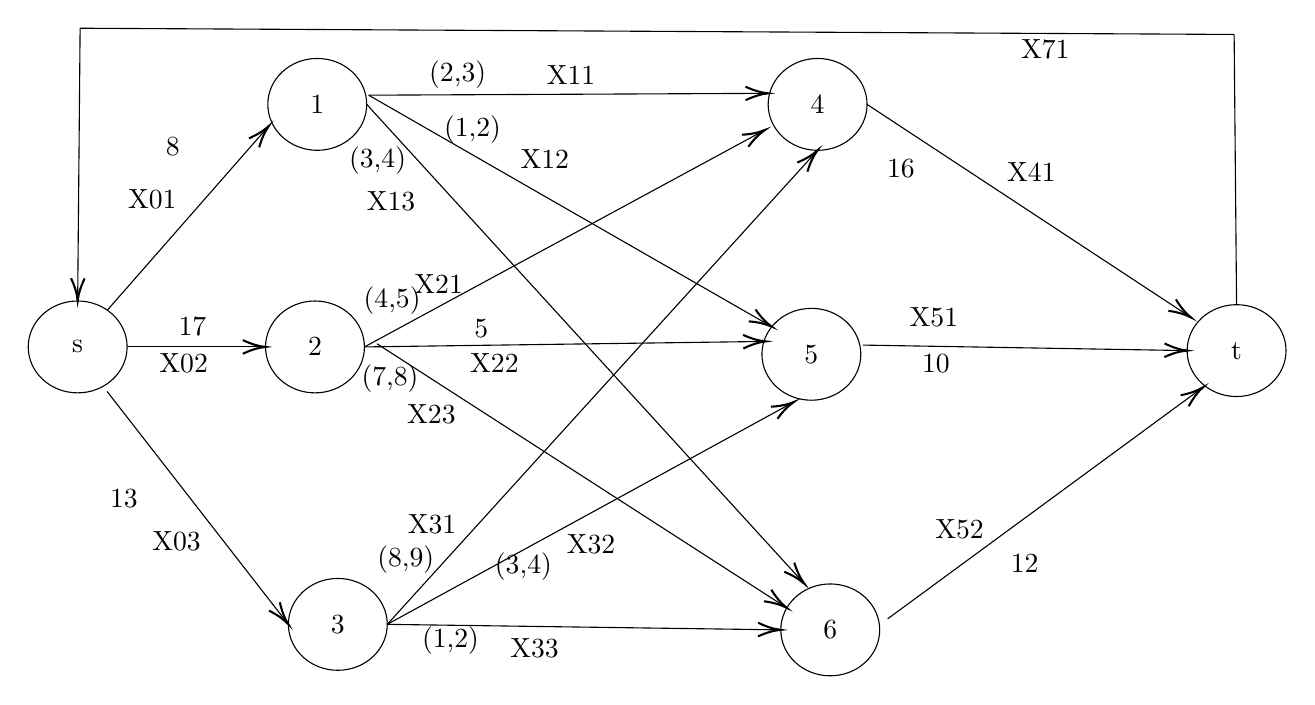
\begin{tikzpicture}[x=0.75pt,y=0.75pt,yscale=-1,xscale=1]
%uncomment if require: \path (0,328); %set diagram left start at 0, and has height of 328

%Shape: Ellipse [id:dp6087199415982871] 
\draw   (5,164.55) .. controls (5,152.33) and (15.66,142.42) .. (28.82,142.42) .. controls (41.98,142.42) and (52.64,152.33) .. (52.64,164.55) .. controls (52.64,176.77) and (41.98,186.68) .. (28.82,186.68) .. controls (15.66,186.68) and (5,176.77) .. (5,164.55) -- cycle ;
%Shape: Ellipse [id:dp6442628638464488] 
\draw   (120.43,47.69) .. controls (120.43,35.46) and (131.1,25.56) .. (144.25,25.56) .. controls (157.41,25.56) and (168.08,35.46) .. (168.08,47.69) .. controls (168.08,59.91) and (157.41,69.82) .. (144.25,69.82) .. controls (131.1,69.82) and (120.43,59.91) .. (120.43,47.69) -- cycle ;
%Shape: Ellipse [id:dp1061001134607138] 
\draw   (119.34,164.55) .. controls (119.34,152.33) and (130,142.42) .. (143.16,142.42) .. controls (156.32,142.42) and (166.98,152.33) .. (166.98,164.55) .. controls (166.98,176.77) and (156.32,186.68) .. (143.16,186.68) .. controls (130,186.68) and (119.34,176.77) .. (119.34,164.55) -- cycle ;
%Shape: Ellipse [id:dp07911004918526843] 
\draw   (130.34,298.21) .. controls (130.34,285.99) and (141,276.09) .. (154.16,276.09) .. controls (167.32,276.09) and (177.98,285.99) .. (177.98,298.21) .. controls (177.98,310.44) and (167.32,320.34) .. (154.16,320.34) .. controls (141,320.34) and (130.34,310.44) .. (130.34,298.21) -- cycle ;
%Shape: Ellipse [id:dp03846588488001945] 
\draw   (361.5,47.69) .. controls (361.5,35.46) and (372.16,25.56) .. (385.32,25.56) .. controls (398.48,25.56) and (409.14,35.46) .. (409.14,47.69) .. controls (409.14,59.91) and (398.48,69.82) .. (385.32,69.82) .. controls (372.16,69.82) and (361.5,59.91) .. (361.5,47.69) -- cycle ;
%Shape: Ellipse [id:dp6541338138904766] 
\draw   (358.5,168.09) .. controls (358.5,155.87) and (369.16,145.96) .. (382.32,145.96) .. controls (395.48,145.96) and (406.14,155.87) .. (406.14,168.09) .. controls (406.14,180.31) and (395.48,190.22) .. (382.32,190.22) .. controls (369.16,190.22) and (358.5,180.31) .. (358.5,168.09) -- cycle ;
%Shape: Ellipse [id:dp4549789345673577] 
\draw   (367.59,300.87) .. controls (367.59,288.65) and (378.26,278.74) .. (391.42,278.74) .. controls (404.57,278.74) and (415.24,288.65) .. (415.24,300.87) .. controls (415.24,313.09) and (404.57,323) .. (391.42,323) .. controls (378.26,323) and (367.59,313.09) .. (367.59,300.87) -- cycle ;
%Shape: Ellipse [id:dp8272562609322014] 
\draw   (563.36,166.32) .. controls (563.36,154.1) and (574.02,144.19) .. (587.18,144.19) .. controls (600.34,144.19) and (611,154.1) .. (611,166.32) .. controls (611,178.54) and (600.34,188.45) .. (587.18,188.45) .. controls (574.02,188.45) and (563.36,178.54) .. (563.36,166.32) -- cycle ;
%Straight Lines [id:da9018286841586965] 
\draw    (43.11,146.84) -- (119.68,59.5) ;
\draw [shift={(121,58)}, rotate = 491.24] [color={rgb, 255:red, 0; green, 0; blue, 0 }  ][line width=0.75]    (10.93,-3.29) .. controls (6.95,-1.4) and (3.31,-0.3) .. (0,0) .. controls (3.31,0.3) and (6.95,1.4) .. (10.93,3.29)   ;

%Straight Lines [id:da06248575236412646] 
\draw    (52.64,164.55) -- (117.34,164.55) ;
\draw [shift={(119.34,164.55)}, rotate = 180] [color={rgb, 255:red, 0; green, 0; blue, 0 }  ][line width=0.75]    (10.93,-3.29) .. controls (6.95,-1.4) and (3.31,-0.3) .. (0,0) .. controls (3.31,0.3) and (6.95,1.4) .. (10.93,3.29)   ;

%Straight Lines [id:da3422343152189683] 
\draw    (43,186) -- (129.11,296.64) ;
\draw [shift={(130.34,298.21)}, rotate = 232.11] [color={rgb, 255:red, 0; green, 0; blue, 0 }  ][line width=0.75]    (10.93,-3.29) .. controls (6.95,-1.4) and (3.31,-0.3) .. (0,0) .. controls (3.31,0.3) and (6.95,1.4) .. (10.93,3.29)   ;

%Straight Lines [id:da7764471766115765] 
\draw    (168.08,47.69) -- (377.68,277.26) ;
\draw [shift={(379.03,278.74)}, rotate = 227.6] [color={rgb, 255:red, 0; green, 0; blue, 0 }  ][line width=0.75]    (10.93,-3.29) .. controls (6.95,-1.4) and (3.31,-0.3) .. (0,0) .. controls (3.31,0.3) and (6.95,1.4) .. (10.93,3.29)   ;

%Straight Lines [id:da6708148744128288] 
\draw    (169.03,43.26) -- (359.5,42.38) ;
\draw [shift={(361.5,42.37)}, rotate = 539.74] [color={rgb, 255:red, 0; green, 0; blue, 0 }  ][line width=0.75]    (10.93,-3.29) .. controls (6.95,-1.4) and (3.31,-0.3) .. (0,0) .. controls (3.31,0.3) and (6.95,1.4) .. (10.93,3.29)   ;

%Straight Lines [id:da04844893541614448] 
\draw    (169.03,43.26) -- (361.53,153.82) ;
\draw [shift={(363.26,154.81)}, rotate = 209.87] [color={rgb, 255:red, 0; green, 0; blue, 0 }  ][line width=0.75]    (10.93,-3.29) .. controls (6.95,-1.4) and (3.31,-0.3) .. (0,0) .. controls (3.31,0.3) and (6.95,1.4) .. (10.93,3.29)   ;

%Straight Lines [id:da603114895121129] 
\draw    (166.98,164.55) -- (358.24,60.95) ;
\draw [shift={(360,60)}, rotate = 511.56] [color={rgb, 255:red, 0; green, 0; blue, 0 }  ][line width=0.75]    (10.93,-3.29) .. controls (6.95,-1.4) and (3.31,-0.3) .. (0,0) .. controls (3.31,0.3) and (6.95,1.4) .. (10.93,3.29)   ;

%Straight Lines [id:da2515352222135493] 
\draw    (166.98,164.55) -- (358.41,161.92) ;
\draw [shift={(360.41,161.89)}, rotate = 539.21] [color={rgb, 255:red, 0; green, 0; blue, 0 }  ][line width=0.75]    (10.93,-3.29) .. controls (6.95,-1.4) and (3.31,-0.3) .. (0,0) .. controls (3.31,0.3) and (6.95,1.4) .. (10.93,3.29)   ;

%Straight Lines [id:da18679069580618912] 
\draw    (173,163) -- (368.77,289.16) ;
\draw [shift={(370.45,290.25)}, rotate = 212.8] [color={rgb, 255:red, 0; green, 0; blue, 0 }  ][line width=0.75]    (10.93,-3.29) .. controls (6.95,-1.4) and (3.31,-0.3) .. (0,0) .. controls (3.31,0.3) and (6.95,1.4) .. (10.93,3.29)   ;

%Straight Lines [id:da5352286234985627] 
\draw    (177.98,298.21) -- (383.98,71.3) ;
\draw [shift={(385.32,69.82)}, rotate = 492.23] [color={rgb, 255:red, 0; green, 0; blue, 0 }  ][line width=0.75]    (10.93,-3.29) .. controls (6.95,-1.4) and (3.31,-0.3) .. (0,0) .. controls (3.31,0.3) and (6.95,1.4) .. (10.93,3.29)   ;

%Straight Lines [id:da24470161199444096] 
\draw    (177.98,298.21) -- (372.25,191.96) ;
\draw [shift={(374,191)}, rotate = 511.32] [color={rgb, 255:red, 0; green, 0; blue, 0 }  ][line width=0.75]    (10.93,-3.29) .. controls (6.95,-1.4) and (3.31,-0.3) .. (0,0) .. controls (3.31,0.3) and (6.95,1.4) .. (10.93,3.29)   ;

%Straight Lines [id:da9109780361808164] 
\draw    (177.98,298.21) -- (365.59,300.84) ;
\draw [shift={(367.59,300.87)}, rotate = 180.8] [color={rgb, 255:red, 0; green, 0; blue, 0 }  ][line width=0.75]    (10.93,-3.29) .. controls (6.95,-1.4) and (3.31,-0.3) .. (0,0) .. controls (3.31,0.3) and (6.95,1.4) .. (10.93,3.29)   ;

%Straight Lines [id:da7064833162794362] 
\draw    (419.05,295.56) -- (569.39,185.18) ;
\draw [shift={(571,184)}, rotate = 503.71] [color={rgb, 255:red, 0; green, 0; blue, 0 }  ][line width=0.75]    (10.93,-3.29) .. controls (6.95,-1.4) and (3.31,-0.3) .. (0,0) .. controls (3.31,0.3) and (6.95,1.4) .. (10.93,3.29)   ;

%Straight Lines [id:da09223774664487527] 
\draw    (409.14,47.69) -- (563.59,149.29) ;
\draw [shift={(565.26,150.39)}, rotate = 213.34] [color={rgb, 255:red, 0; green, 0; blue, 0 }  ][line width=0.75]    (10.93,-3.29) .. controls (6.95,-1.4) and (3.31,-0.3) .. (0,0) .. controls (3.31,0.3) and (6.95,1.4) .. (10.93,3.29)   ;

%Straight Lines [id:da3088611575507132] 
\draw    (407.09,163.66) -- (561.36,166.28) ;
\draw [shift={(563.36,166.32)}, rotate = 180.97] [color={rgb, 255:red, 0; green, 0; blue, 0 }  ][line width=0.75]    (10.93,-3.29) .. controls (6.95,-1.4) and (3.31,-0.3) .. (0,0) .. controls (3.31,0.3) and (6.95,1.4) .. (10.93,3.29)   ;

%Straight Lines [id:da4881283804502492] 
\draw    (586,14) -- (587.18,144.19) ;


%Straight Lines [id:da3505876176513657] 
\draw    (30,11) -- (586,14) ;


%Straight Lines [id:da7612042307271581] 
\draw    (30,11) -- (28.84,140.42) ;
\draw [shift={(28.82,142.42)}, rotate = 270.51] [color={rgb, 255:red, 0; green, 0; blue, 0 }  ][line width=0.75]    (10.93,-3.29) .. controls (6.95,-1.4) and (3.31,-0.3) .. (0,0) .. controls (3.31,0.3) and (6.95,1.4) .. (10.93,3.29)   ;


% Text Node
\draw (587.18,166.32) node  [align=left] {t};
% Text Node
\draw (28.82,164.55) node  [align=left] {s};
% Text Node
\draw (74.7,68.04) node  [align=left] {8};
% Text Node
\draw (84.08,154.81) node  [align=left] {17};
% Text Node
\draw (51.08,237.5) node  [align=left] {13};
% Text Node
\draw (211.91,33.52) node  [align=left] {(2,3)};
% Text Node
\draw (219.06,59.88) node  [align=left] {(1,2)};
% Text Node
\draw (173.32,74.89) node  [align=left] {(3,4)};
% Text Node
\draw (485.12,268.82) node  [align=left] {12};
% Text Node
\draw (180.32,142.42) node  [align=left] {(4,5)};
% Text Node
\draw (223.25,155.58) node  [align=left] {5};
% Text Node
\draw (179.32,179.8) node  [align=left] {(7,8)};
% Text Node
\draw (186.87,267.24) node  [align=left] {(8,9)};
% Text Node
\draw (243.58,270.54) node  [align=left] {(3,4)};
% Text Node
\draw (208.47,306.18) node  [align=left] {(1,2)};
% Text Node
\draw (442.35,172.51) node  [align=left] {10};
% Text Node
\draw (425.49,78.47) node  [align=left] {16};
% Text Node
\draw (144.25,47.69) node  [align=left] {1};
% Text Node
\draw (391.42,300.87) node  [align=left] {6};
% Text Node
\draw (385.32,47.69) node  [align=left] {4};
% Text Node
\draw (143.16,164.55) node  [align=left] {2};
% Text Node
\draw (382.32,168.09) node  [align=left] {5};
% Text Node
\draw (154.16,298.21) node  [align=left] {3};
% Text Node
\draw (266.54,33.34) node  [align=left] {X11};
% Text Node
\draw (76.47,258.28) node  [align=left] {X03};
% Text Node
\draw (79.87,172.23) node  [align=left] {X02};
% Text Node
\draw (64.74,93.18) node  [align=left] {X01};
% Text Node
\draw (453.73,252.16) node  [align=left] {X52};
% Text Node
\draw (441.37,149.99) node  [align=left] {X51};
% Text Node
\draw (488.35,80.38) node  [align=left] {X41};
% Text Node
\draw (248.98,309.65) node  [align=left] {X33};
% Text Node
\draw (276.19,259.3) node  [align=left] {X32};
% Text Node
\draw (199.52,250.05) node  [align=left] {X31};
% Text Node
\draw (199.24,197.03) node  [align=left] {X23};
% Text Node
\draw (229.62,172.23) node  [align=left] {X22};
% Text Node
\draw (202.75,134.42) node  [align=left] {X21};
% Text Node
\draw (179.84,94.17) node  [align=left] {X13};
% Text Node
\draw (253.86,73.82) node  [align=left] {X12};
% Text Node
\draw (495,21) node  [align=left] {X71};


\end{tikzpicture}

    \caption{Example matrix turned into a maximum flow ciculation problem}
    \label{fig:circulationmaxflow}
\end{figure}
\section*{Task 3 - Implementation}

I modelled this in GLPK using C, I started out by calculating the row and column sums and claculating the number of constraints and variables. Then I set the objective function and set GLPK to maximise. After this I created all the constraints, when I first attempted this I tried to create the constraints in a way that they would work for any sized matrix. I was not able to completely do this, the edge constraints should work for any sized matrix but the node constraints will not. Putting the output value into the matrix will also only work for a 3x3 matrix. 

The variables are marked as being unbounded because by default they were marked as being equal to 0 and this obviously causes the problem to be unsolvable. The constraints are what mark the variable as being bounded between two values.

From a software engineering point of view I've written some comments and made the code somewhat usable for different sized matrices. My implementation works for all the example inputs that are 3x3. 

I would of liked to implement my model in a way that allowed it to work with any sized matrix but implementing that with my node constraints is something that I cannot currently make work.

\section*{Task 4 - Discussion and Conclusion}

The implementation of my approach works for a matrix that is 3x3 and my model works for the first 4 test files provided. I'm quite happy with my end result and the approach I took, obviously I would of liked for my program to deal with any sized matrix and my model allows for this to work. However I am unsure how to implement the node constraints for this in C.

If I were to solve this problem again I would not use linear programming because it's easier to solve it in a numerical way, if for each value in the matrix you take the lower bound value away from its row and column sum. Consider the matrix shown in table \ref{tab:matrix}, for example for the first row you would do 16-2-4-8 = 2. you do this for every row and column and end up with the matrix shown in table \ref{tab:matrixaftersubtraction}, then you fill the matrix with 1s and 0s and this is shown in table \ref{tab:matrixaftersubtractionwithplacements}, if at this stage you cannot form a matrix that adheres to this then there isn't valid rounding for that problem. You then add the lower bounds back into the matrix at their original positions, table \ref{tab:matrixsolved} shows the matrix solved this way.

This is easier then using a linear programming approach and it would allow you to solve the problem in other languages that didn't have a linear programming solver. It would also mean you wouldn't have to construct a maximum flow problem. However if I needed to solve a maximum flow problem in the future I would definitely use linear programming because this approach works incredibly well and is easier than other methods, constructing rules and constraints for your problem is already something you mentally do when solving a complex problem, with linear programming you're just applying those rules in a different way.

I'd give myself a mark of around 65-70/100 because my model works to solve this problem and I've written code to prove it, however this only works for 3x3 matrices so I am loosing marks there. It might fail for all the additional test files because they could all be bigger matrices so I'm not expecting any marks there, but I'm confident with the content of my report and I feel that my model is robust and correct.

\begin{table}[]
\centering
\begin{tabular}{|l|l|l|l|}
\hline
2.9 & 4.6 & 8.5 & 16 \\ \hline
1.9 & 5   & 3.1 & 10 \\ \hline
3.2 & 7.4 & 1.4 & 12 \\ \hline
8   & 17  & 13  &    \\ \hline
\end{tabular}
\caption{The example matrix.}
\label{tab:matrix}
\end{table}

\begin{table}[]
\centering
\begin{tabular}{|l|l|l|l|}
\hline
  &   &   & 2 \\ \hline
  &   &   & 1 \\ \hline
  &   &   & 1 \\ \hline
2 & 1 & 1 &   \\ \hline
\end{tabular}
\caption{The example matrix after subtracting the lower bounds from the row and column totals.}
\label{tab:matrixaftersubtraction}
\end{table}

\begin{table}[]
\centering
\begin{tabular}{|l|l|l|l|}
\hline
1 & 1 & 0 & 2 \\ \hline
1 & 0 & 0 & 1 \\ \hline
0 & 0 & 1 & 1 \\ \hline
2 & 1 & 1 &   \\ \hline
\end{tabular}
\caption{The example matrix after subtracting the lower bounds from the row and column totals and with 1s and 0s added in to produce a valid matrix.}
\label{tab:matrixaftersubtractionwithplacements}
\end{table}

\begin{table}[]
\centering
\begin{tabular}{|l|l|l|l|}
\hline
3 & 5  & 8  & 16 \\ \hline
2 & 5  & 3  & 10 \\ \hline
3 & 7  & 2  & 12 \\ \hline
8 & 17 & 13 &    \\ \hline
\end{tabular}
\caption{The example matrix solved using a numerical method.}
\label{tab:matrixsolved}
\end{table}

\bibliographystyle{plain}
\nocite{*}
\bibliography{bib.bib}

\end{document}  
%%%%%%%%%%%%%%%%%%%%%%%%%%%%%%%%%%%%%%%%%%%%%%